%
% common information to the web version and book version
%
% images will be imported by searching the paths set with \graphicspath
% the book.tex or web.tex sets this so the correct resolution images end
% up in the correct document.
% 
% cover is done elsewhere, as this is usually broken out from the 
% ``text block'' for POD publishing--see book.tex
%

\vspace*{5in}
{\large Copyright (C) 2009 Lu Tao  All Rights Reserved.}

This book may not be reproduced in any form without written permission
of the author. 

{\tt 1417274896@qq.com}
\newpage

\vspace*{2in}
\begin{center}
{\LARGE For You}

{\large For auld lang syne}

\vspace*{0.5in}

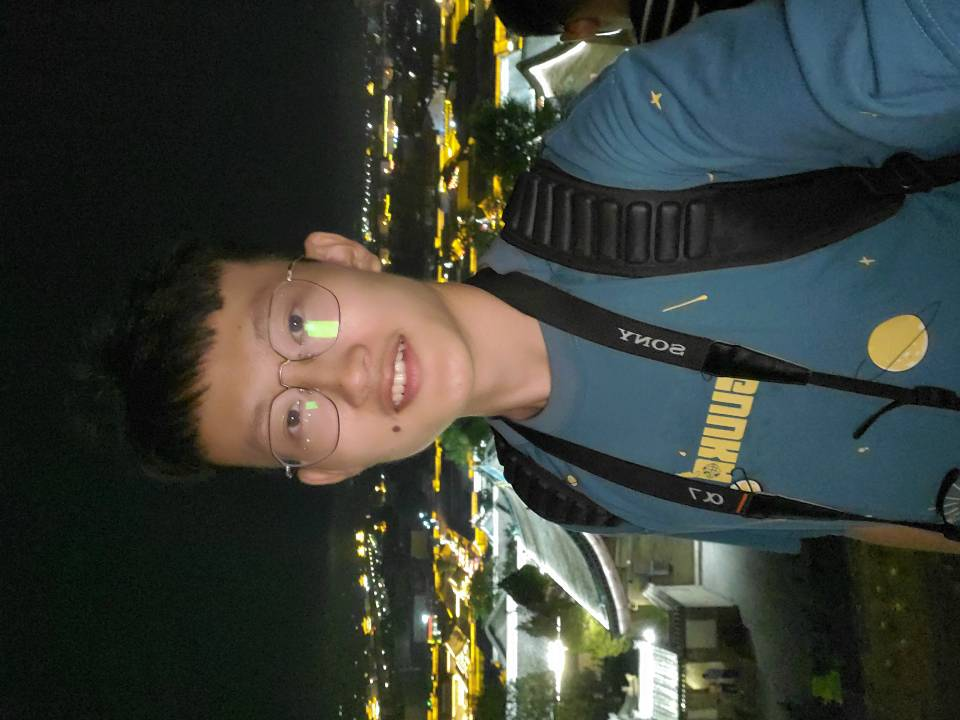
\includegraphics[width=3in]{me_night.jpg}
\end{center}
\newpage

\vspace*{1in}
{\LARGE About this book}

I'm writing this book to practise {LaTeX} skills.


\vspace*{0.25in}

{\LARGE This boy is from the steppe.}

This boy is from the steppe.
I've speed most of my childhood in Hohhot, Inner Mongolia. 
The scene of the steppe in my hometown keeps flashing back in my mind these days.  
And it inspires me to make this album in memory of my past days.
These photographs represent some part of me. 
To some extent, to read this book is to read about this boy.

It's 20th May. My birthday is just around the corner.
Maybe I just want to make a gift myself.

25th May updates.
I though about the meaning of love, perpose of human beings, 
progress in policy and many and many abstruct things.
What emerge in my thoughts force me to construct my mind and keep thinking.
But I cannot convince myself in the end.
Just like a undamped oscillation procedure with a damping of $-\infty$ .

Light, shadow, and color composed my visual world. 

% {\Large {\em BacGawwwwk!!}} %����
\newpage

\vspace*{3in}
\begin{center}
\Huge{There's a hint of summer in the air.}
\end{center}
\newpage

\pagestyle{plain}

\vspace*{\fill}
\includegraphics[width=8in]{the70ceremany.jpg}
\textbf{ Culture and Sports Centre }
It was built in 2019. 
The park nearby is enormous and is sparsely populated compared with the QingCheng park.
It's pretty with numerous flowers in summer.
\vspace*{\fill}
\newpage

\vspace*{\fill}
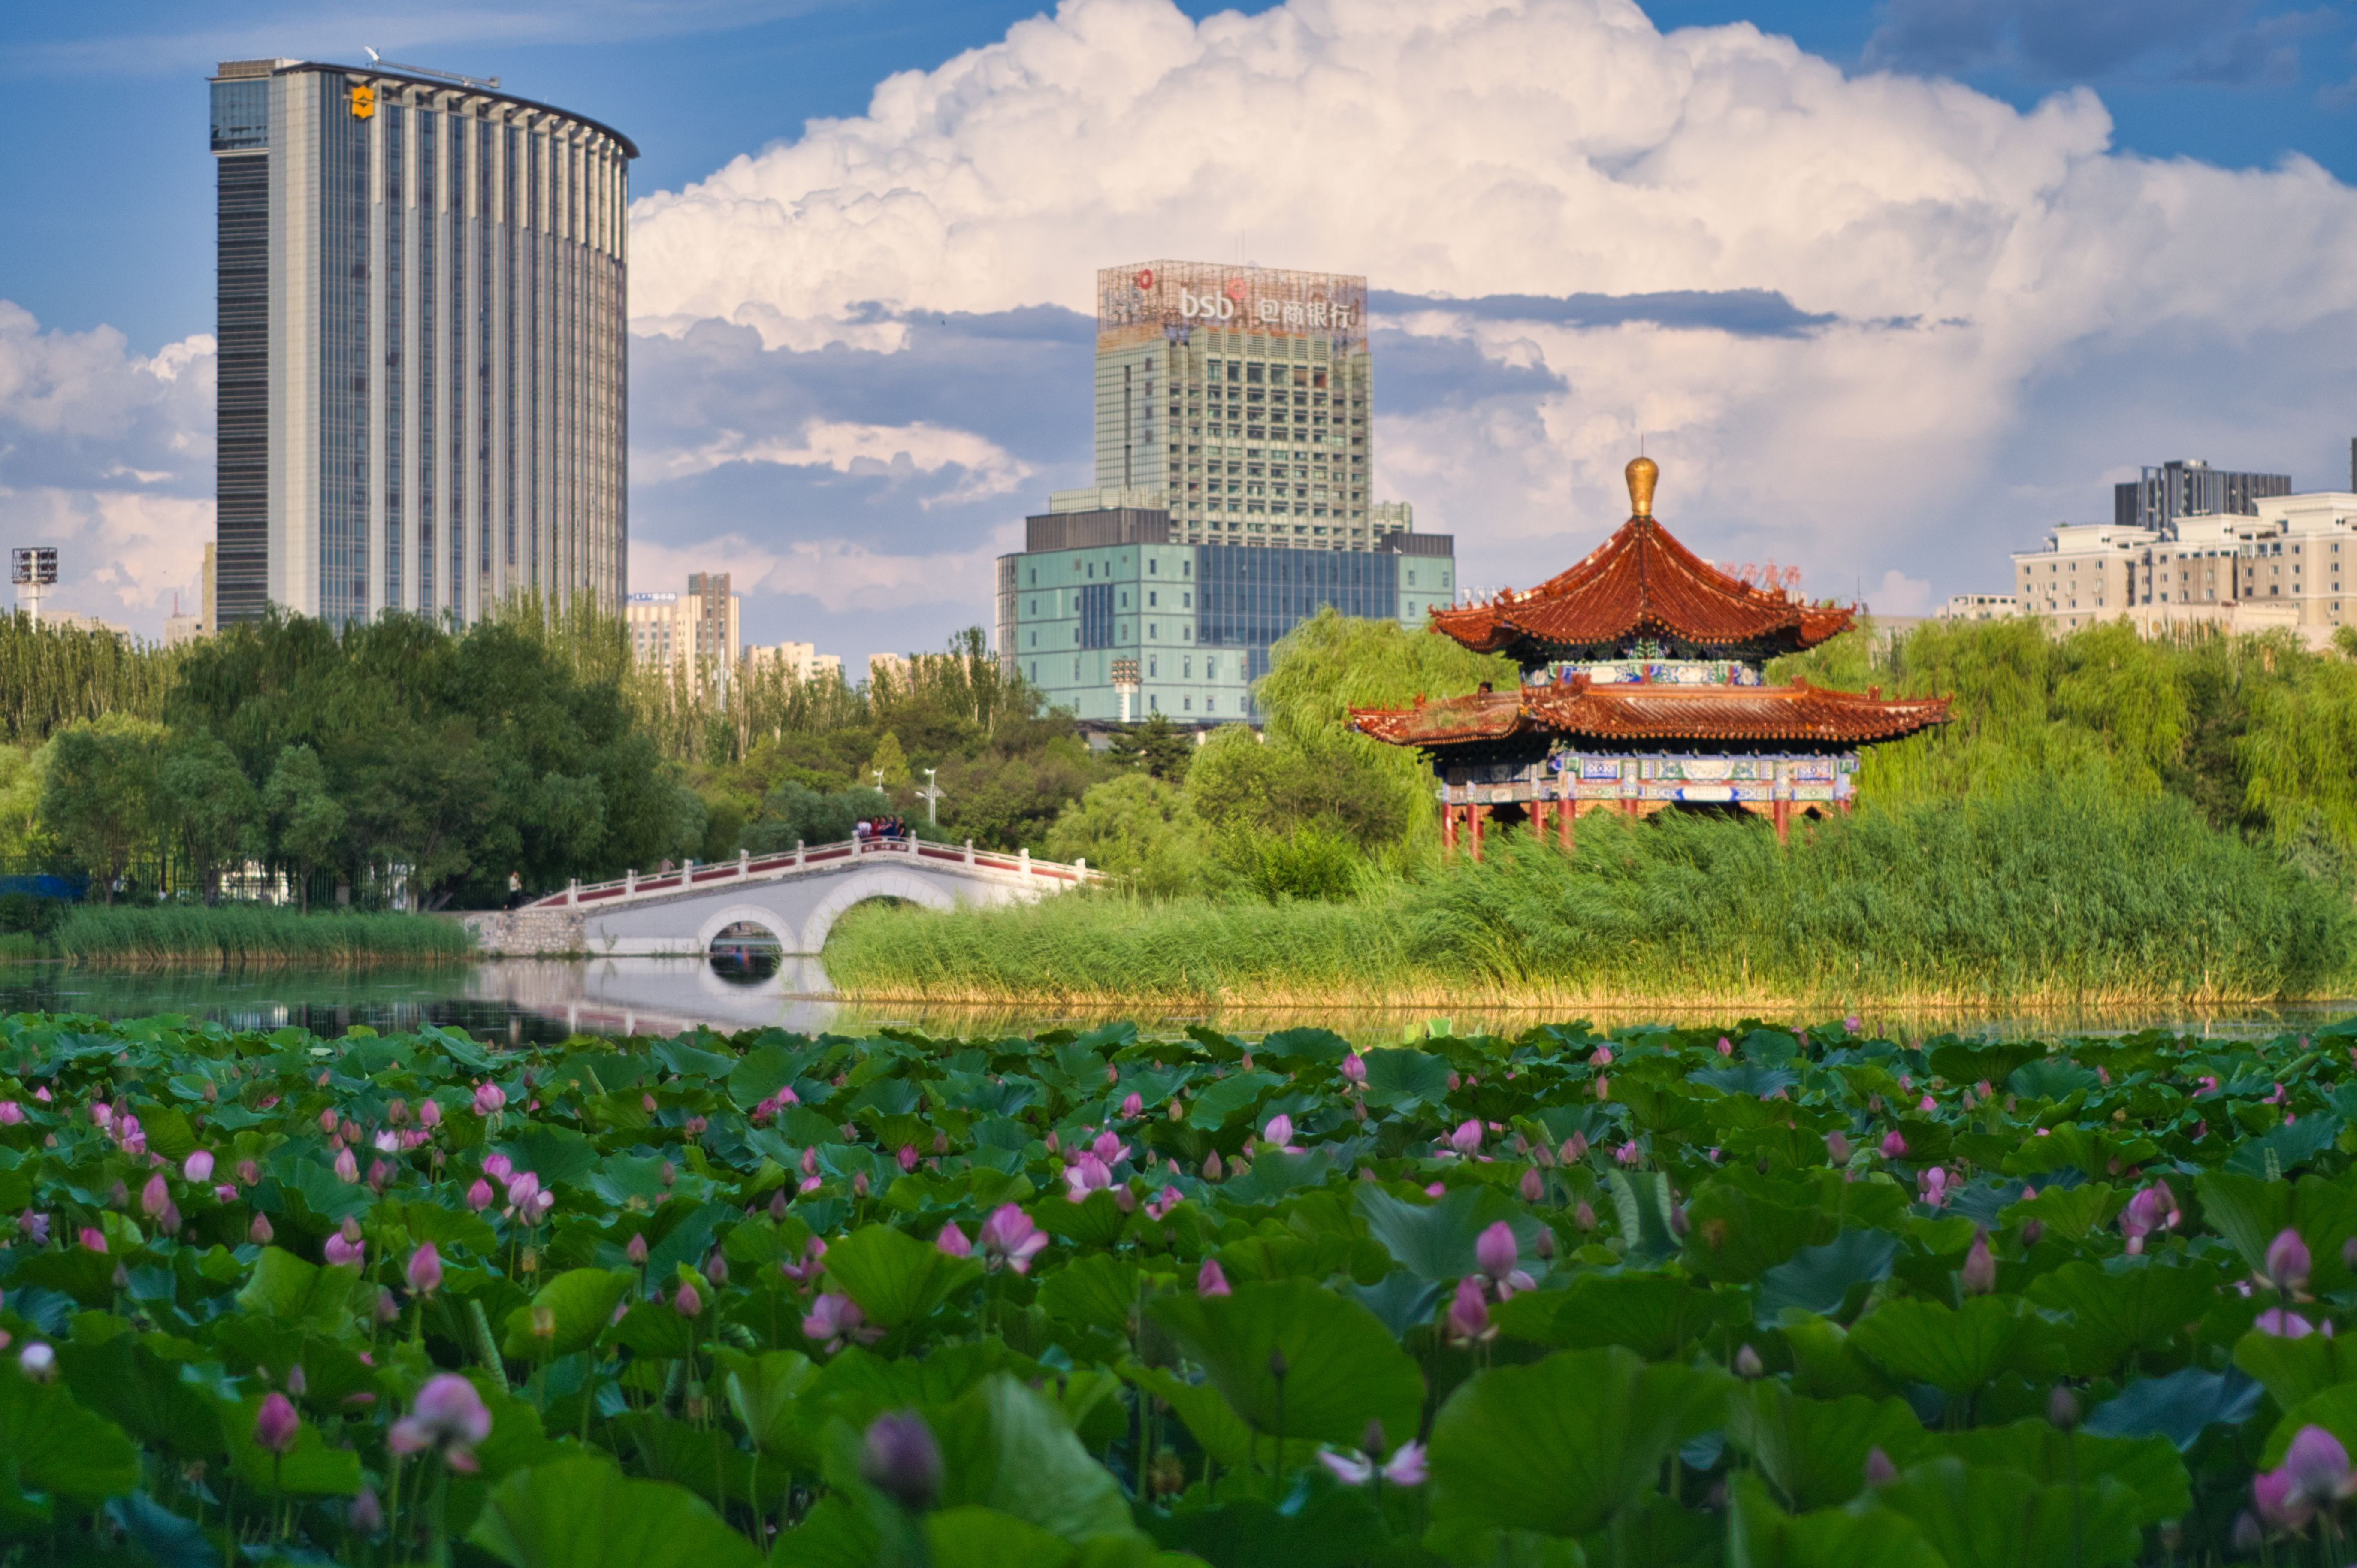
\includegraphics[width=8in]{theQingChengPart.jpg}
\textbf{ QingCheng Park }
It's my most visiting park with flowers in spring, greenery in summer and ice arena in winter. 

\vspace*{\fill}
\newpage

\vspace*{\fill}
\includegraphics[width=8in]{the_Qingcheng_park_lake_in_spring.jpg}
This is one of small ponds in the park. It feels like silk earlier in the summer.
Somehow summer never seems to last long enough. So is my childhood.
\vspace*{\fill}
\newpage

\vspace*{\fill}
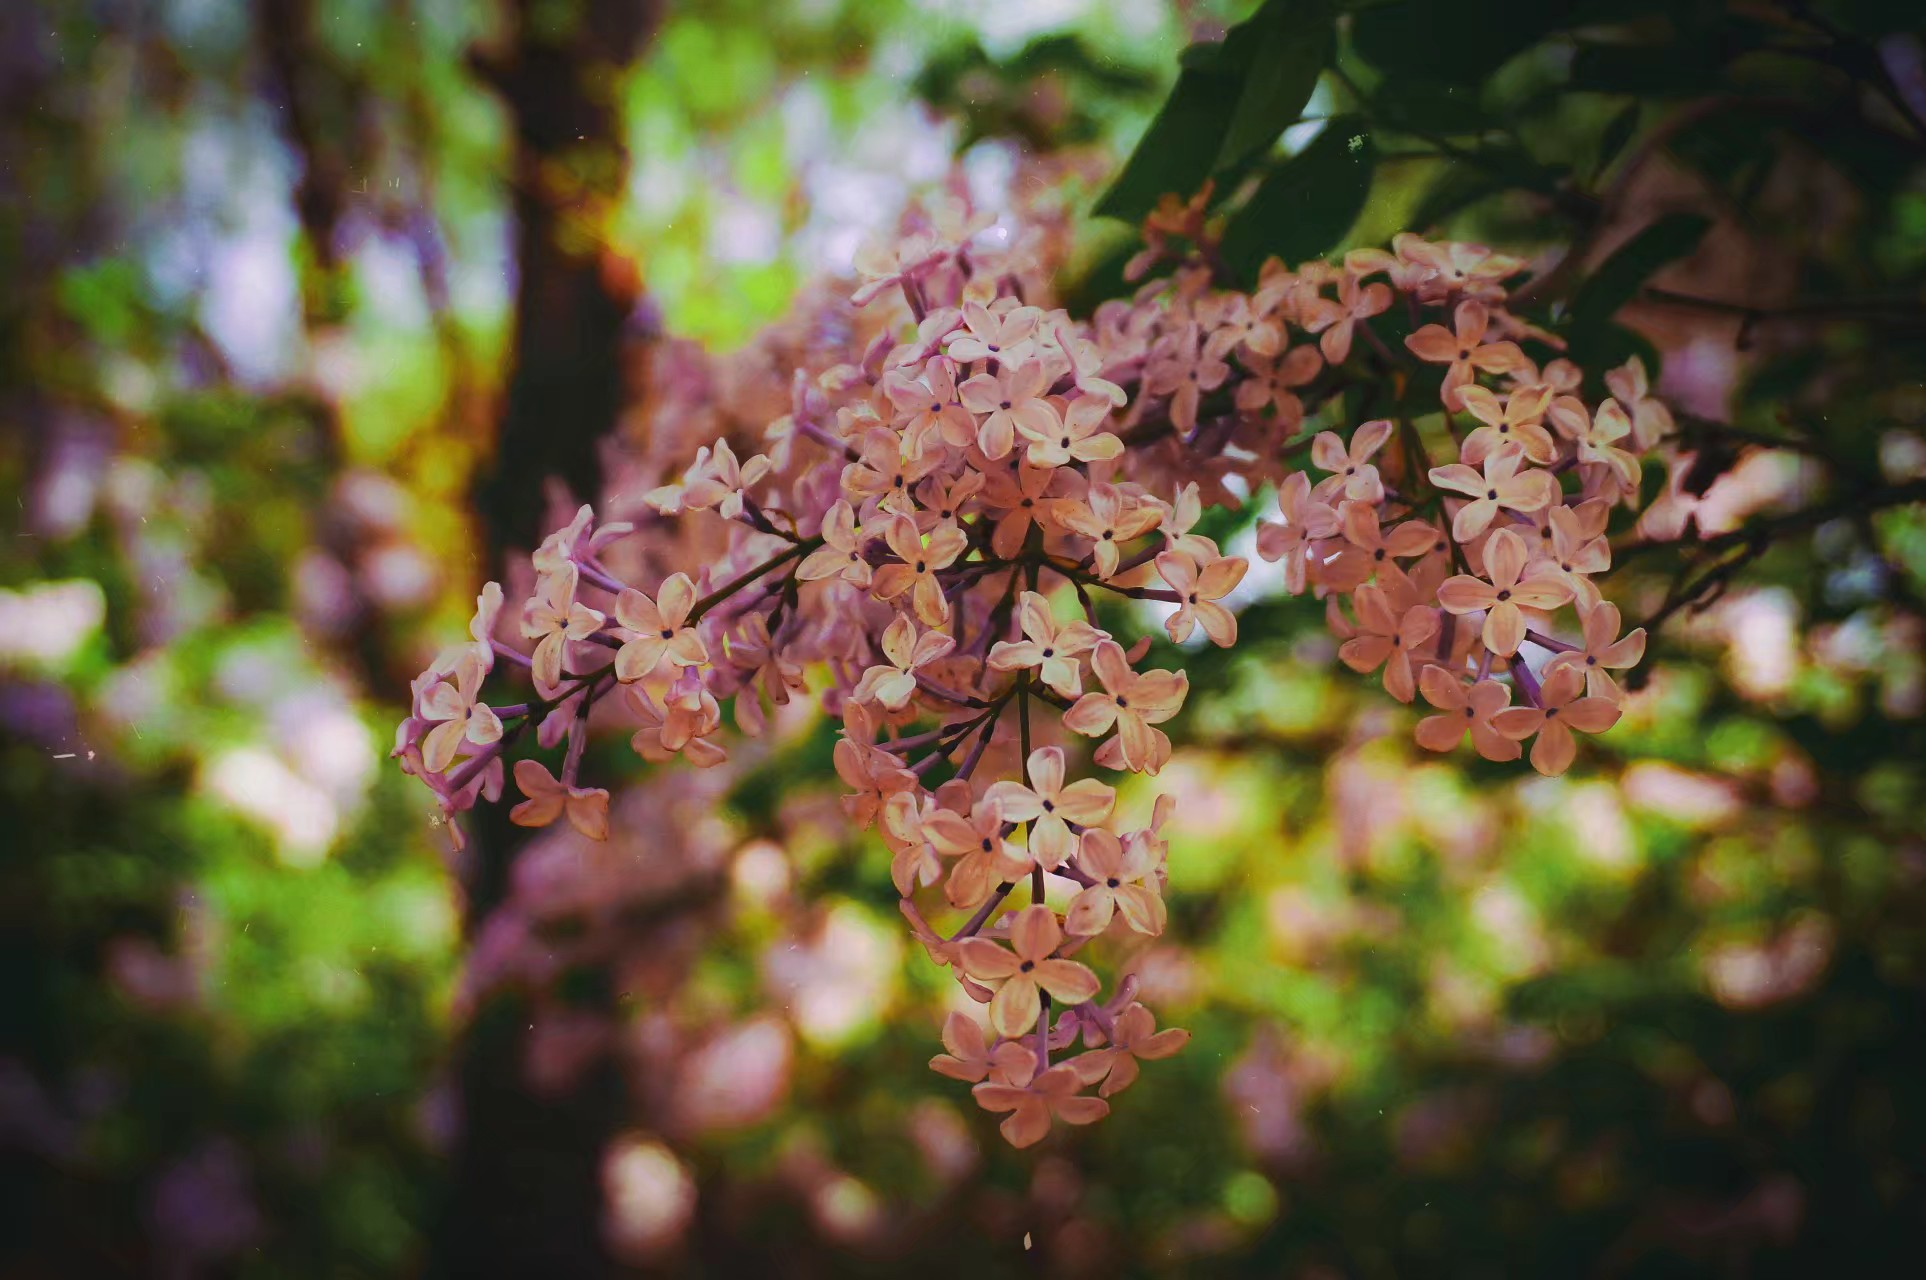
\includegraphics[width=8in]{most_loved_cloves.jpg}
\textbf{Most loved branch of Lilac}
This is my most loved photo when I was a kid. 
I captured it in 2013 and sent it to my best friends immediately. 
The splendid tune of color made me fall in love with photograph. 
\vspace*{\fill}
\newpage

\vspace*{\fill}
\includegraphics[width=8in]{sounder_in_city.jpg}

On a late day in May we headed into town to Del's to pick up the chicks,
\vspace*{\fill}
\newpage

    \vspace*{\fill}
        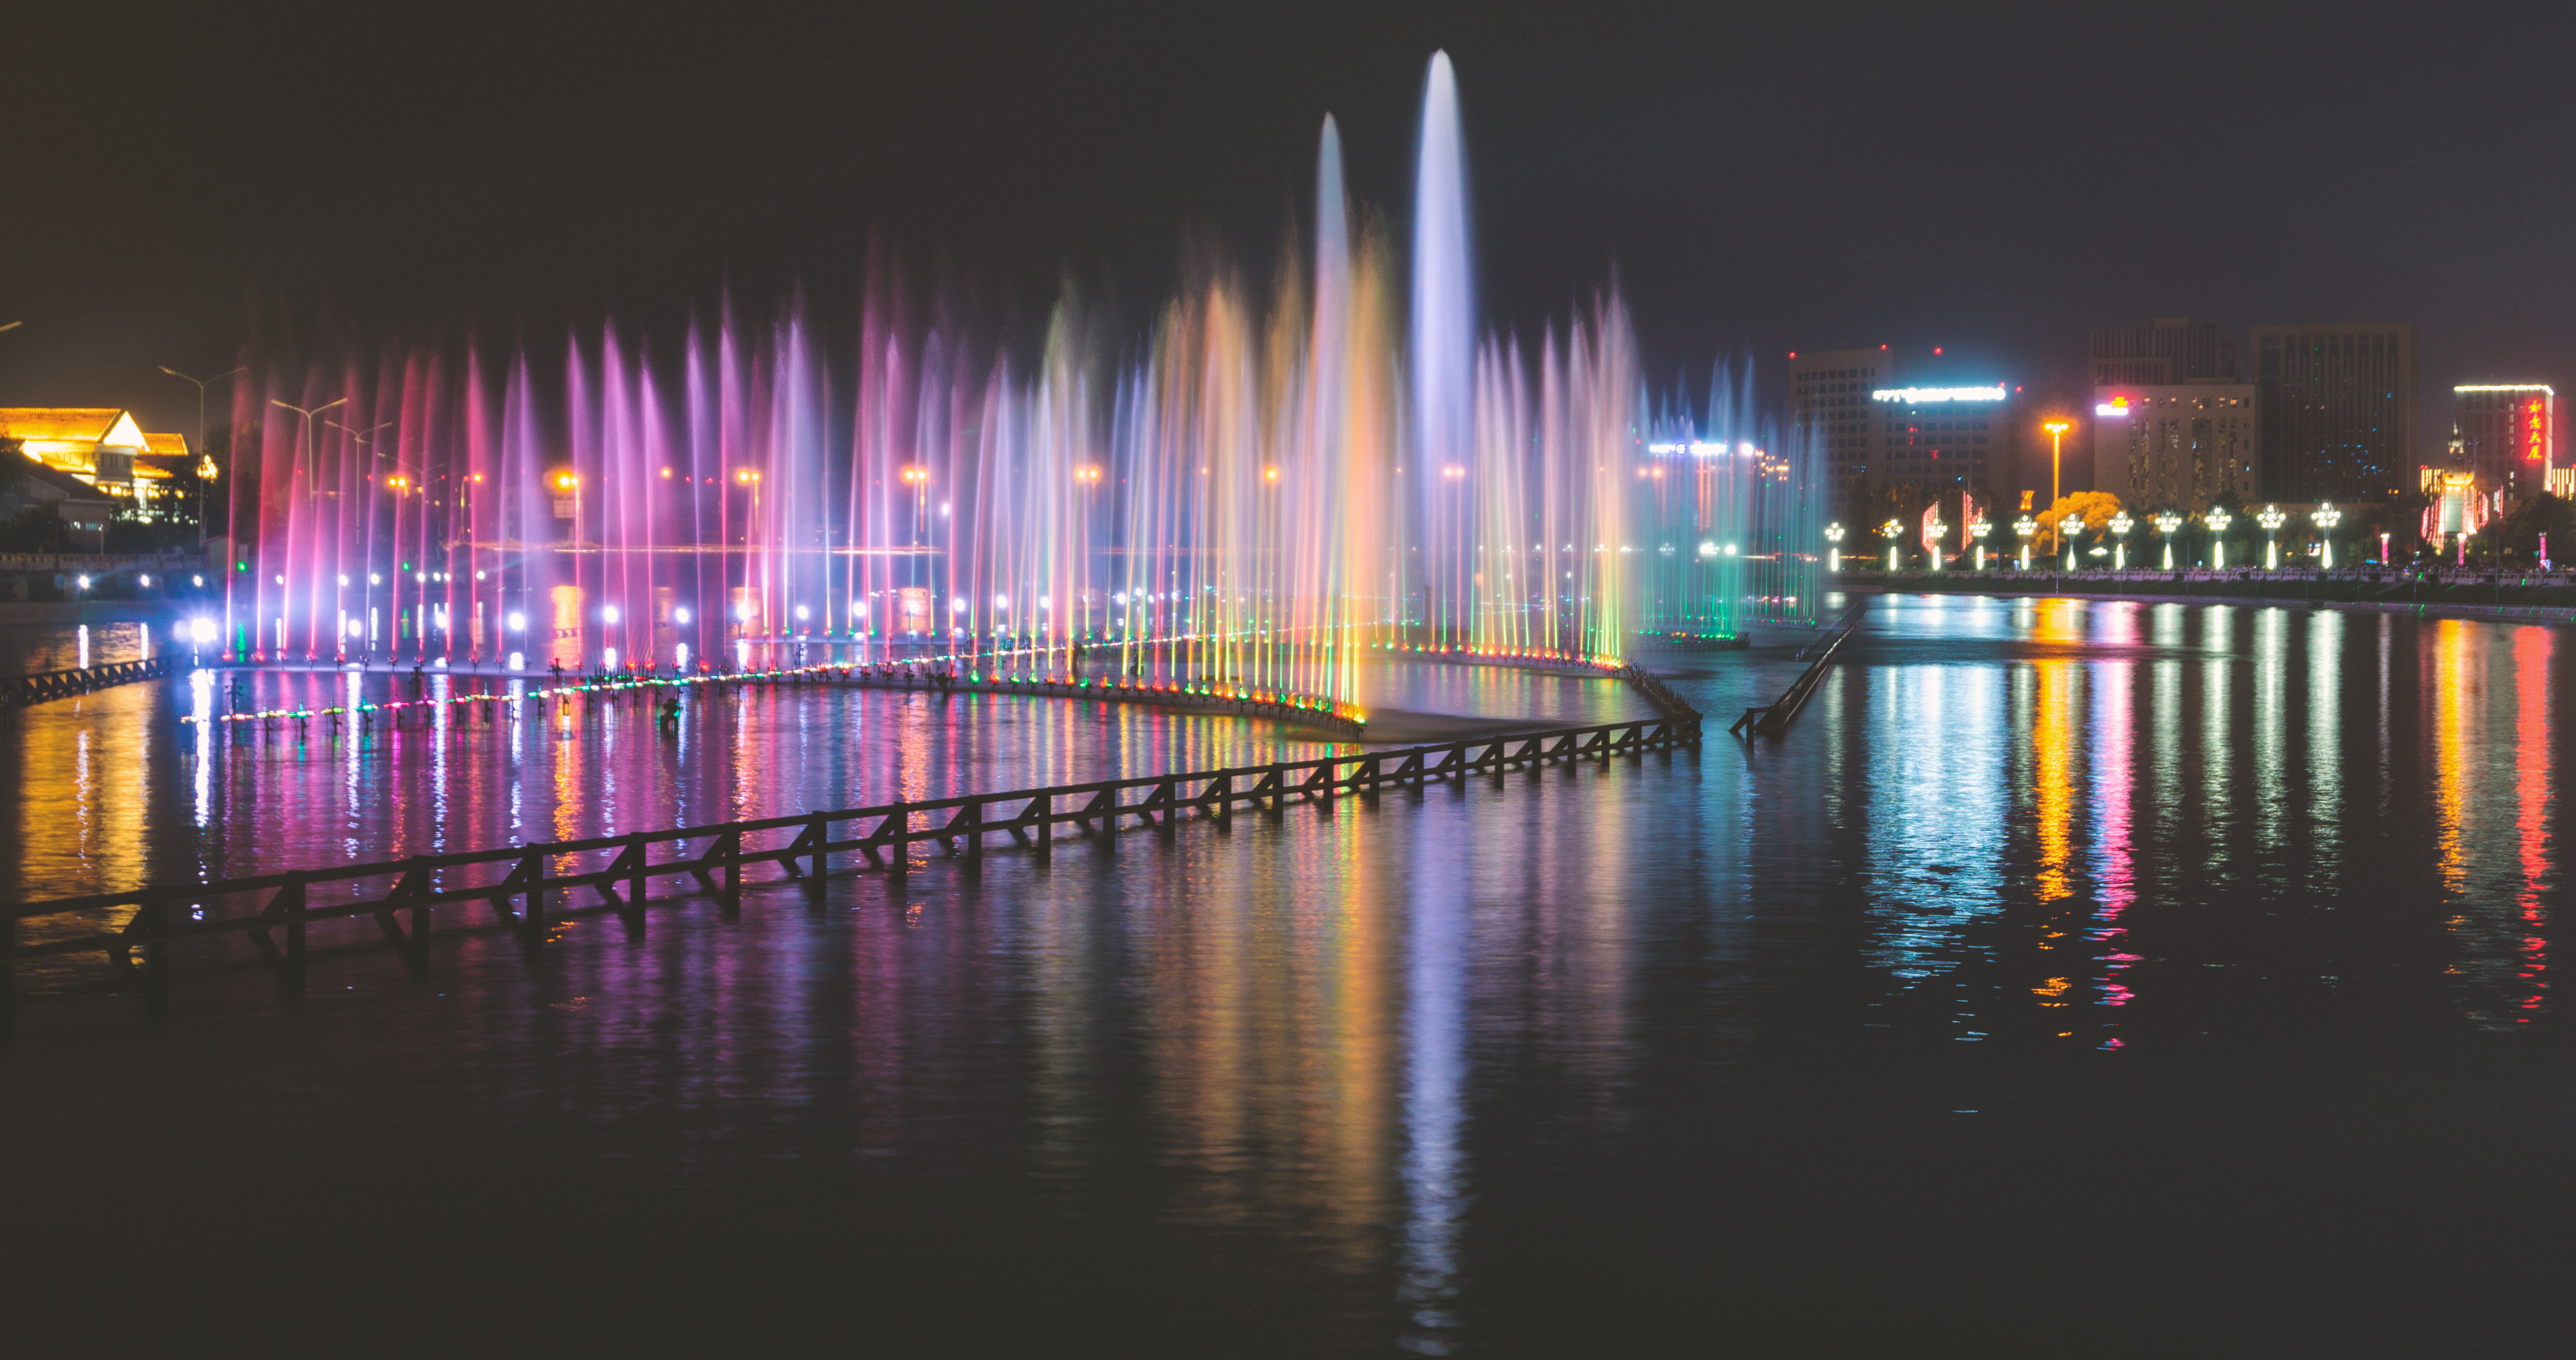
\includegraphics[width=8in]{ruyi_river_fangting}

        Next stop was Home Despot, er, Depot.  I had the beginnings of a plan in
        mind for a chicken coop.  My idea was to use a dog kennel as a starter
        coop.  HD had some inexpensive dog kennel kits, and I knew that with the
        galvanized steel I'd have something that could stand up to the rain, sun
        and termites.  I needed something to keep the chickens in, and predators
        out. 
    \vspace*{\fill}
\newpage

\vspace*{\fill}
\includegraphics[width=8in]{the_grocery}

The 6x6x4 kennel seemed about the right size for 6 chickens, which is
what I was targeting.  My calculations were that six would yield us a
decent number of eggs per week.  After some reconsideration, we put the
\vspace*{\fill}
\newpage

% \begin{center}{\Large ``Furrow'' }\end{center}

\vspace*{1in}

{\LARGE Book Considerations}

Solo Photo Book Month (sofobomo.org) is a DIY project to make a photo
book in one month. All of the photos must be taken and the book laid 
out and processed into a PDF in 31 days. This is my second year
participating in the event, along with many other photographers all over
the world. 
Last year I did square format B\&W, so I was determined to do color and
some sort of rectangular format this year. I chose to go all landscape, 
even though it meant passing on some good verticals I had taken. Also,
last year was more of a series of portraits, and this year I was
determined to have the book tell more of a story. I struggled to find
something that would fit my tight schedule this year when the ``chicken
project'', which I'd had on the back burner, hit me as a good fit to
dovetail with SoFoBoMo. 

If you have a comment to share, thoughts on the book, life with
chickens, technical info, questions, whatever...drop by 

\url{http://redskiesatnight.com/books/chickens-anyone}

and leave a comment. We'd love to hear from you! There you can also
download a PDF version. 

For more information about Solo Photo Book Month, visit

\url{http://sofobomo.org/}

\vspace*{0.25in}

{\LARGE Technical Details}

I was really pressed for time to get the book done in the requisite 30
days this year. I threw it together with snapshots taken with a Ricoh
GX100 camera. No post processing was done except for some quick levels
adjustments in the image editor GIMP.
{\em ImageMagick} was used to batch downsample the images for the web version
(144 dpi) or the book version (300 dpi). 
I designed the book using \LaTeX (with the wonderful {\em xetex} and
{\em xdvipdfmx}) for easier adjustments for dead tree publishing. 
The font used is Garamond. This book was made on Linux.

%END
